
\documentclass[twoside]{article}
\usepackage{CJKutf8}

%\usepackage{graphics}
\usepackage{graphics}
\usepackage{geometry}
\usepackage{forest,amsmath}
\usepackage{enumerate}
\usepackage{url}
\usepackage{latexsym,bm,amssymb}

\geometry{left=2.5cm,right=2cm,top=2.5cm,bottom=2.5cm}

%\setlength{\oddsidemargin}{0.25 in}
%\setlength{\evensidemargin}{-0.25 in}
%\setlength{\topmargin}{-0.6 in}
%\setlength{\textwidth}{6.5 in}
%\setlength{\textheight}{8.5 in}
%\setlength{\headsep}{0.75 in}
\setlength{\parindent}{0 in}
\setlength{\parskip}{0.1 in}

\usepackage{listings}
\usepackage{color}
\renewcommand\lstlistingname{Quelltext} % Change language of section name
\lstset{ % General setup for the package
    language= C,
    %basicstyle=\small\sffamily,
    basicstyle=\ttfamily,
    numbers=left,
     numberstyle=\tiny,
    frame=tb,
    tabsize=4,
    columns=fixed,
    showstringspaces=false,
    showtabs=false,
    keepspaces,
    commentstyle=\color{red},
    keywordstyle=\color{blue}
}

%
% The following commands set up the lecnum (lecture number)
% counter and make various numbering schemes work relative
% to the lecture number.
%
%\newcounter{lecnum}
%\renewcommand{\thepage}{\thelecnum-\arabic{page}}
%\renewcommand{\thesection}{\thelecnum.\arabic{section}}
%\renewcommand{\theequation}{\thelecnum.\arabic{equation}}
%\renewcommand{\thefigure}{\thelecnum.\arabic{figure}}
%\renewcommand{\thetable}{\thelecnum.\arabic{table}}

%
% The following macro is used to generate the header.
%


%


%Use this command for a figure; it puts a figure in wherever you want it.
%usage: 
%\begin{figure}
%\begin{center}
%\includegraphics[width=5in]{fig-file}
%\caption{}\label{fig:delavl}
%\end{center}
%\end{figure}

%%% Use the following command for a table
%%%

% Use these for theorems, lemmas, proofs, etc.
\newtheorem{theorem}{Theorem}[theorem]
\newtheorem{lemma}[theorem]{Lemma}
\newtheorem{proposition}[theorem]{Proposition}
\newtheorem{claim}[theorem]{Claim}
\newtheorem{corollary}[theorem]{Corollary}
\newtheorem{definition}[theorem]{Definition}
\newenvironment{proof}{{\bf Proof:}}{\hfill\rule{2mm}{2mm}}

% **** IF YOU WANT TO DEFINE ADDITIONAL MACROS FOR YOURSELF, PUT THEM HERE:

\begin{document}
\begin{CJK*}{UTF8}{gbsn}
	%FILL IN THE RIGHT INFO.
	%\lecture{**LECTURE-NUMBER**}{**DATE**}{**LECTURER**}{**SCRIBE**}
	%\lecture{1}{Project Name}{Deshi Ye}{Student 1, Student 2, 学生3}
	%\footnotetext{These notes are partially based on those of Nigel Mansell.}
	\title{LC-3 Executor}
	\date{}
	\maketitle
	% **** YOUR NOTES GO HERE:

	% Some general latex examples and examples making use of the
	% macros follow.  
	%**** IN GENERAL, BE BRIEF. LONG SCRIBE NOTES, NO MATTER HOW WELL WRITTEN,
	%**** ARE NEVER READ BY ANYBODY.
	\section{Introduction}
	In this project, we need to write a program to execute LC-3 binary code via \textbf{C} or other high level programming language.
	
	To write the LC-3 executor, we need to implement the instructions like ``BR'', ``ADD'', ``LD'', ``ST'', ``JSR'', ``AND'', ``LDR'', ``STR'', ``NOT'', ``LDI'', ``STI'', ``JMP'', ``LEA''. The only TRAP isntruction we need to implement is HALT instruction, which can stop and exit our executor. Also, the privilege mode, ACV and instructions like RTI, 1101 is not required.
	
	As for registers, the default values of all registers and memory locations are x7777. When the HALT instruction executed by the program, the value of R0,R1,R6 and R7 will remain unchanged, then the program should print the value of all registers.
	
	
	
	\section{Algorithm Specification}
	
	In our program we need to imitate the LC-3 machine to operates the binary code. Therefore, we also need to complete the Instruction Cycle, which includes ``Fetch'', ``Decode'', ``Evaluate Address'', ``Fetch operands'', ``Execute'' and ``Store Result'' six parts.
	
	However, not all instructions will do all parts of the Instructon Cycle. Consequently, we divide the Instruction Cycle into three parts: ``Fetch'', ``Decode'' and ``Execute accordingly''.
	
	\subsection{Data Structure}
	
	To represent a instruction, we define a class called BinaryCode, in which we use a string to represent the binary code and a unsigned int to represent the address of the instruction. Also, there will be some function in the class.
	
	\begin{lstlisting}
	class BinaryCode {
		private:
			string code;
			unsigned short address;
		public:
			......
			
	};
	\end{lstlisting}

	Also, we use a vector to store the instructions inputted and use another vector to serve as a storage of data. Then an array of unsigned int is used to represent the register.
	
	\subsection{Algorithm}
	
	Firstly, we need to process the inputted instruction and store it.
	
	\begin{lstlisting}
		str $\leftarrow$ input
		beginAddr $\leftarrow$ str.transferToDigit()
		while(!EOF)
			str $\leftarrow$ input
			form BinaryCode by str
			store the BinaryCode
	\end{lstlisting}

	
	Then, the program will decode the instructions and process them one by one.
	
	\begin{lstlisting}
	for each instruction i in storage
		opcode = i.getOpcode();
		if (opcode == "0001")add(current_code, nzp_ref);
		if (opcode == "0101")m_and(current_code, nzp_ref);
		if (opcode == "0000")br(current_code, PC_ref, nzp_ref);
		if (opcode == "1100")jump(current_code, PC_ref);
		if (opcode == "0100")jsr(current_code, PC_ref);
		if (opcode == "0010")ld(current_code, PC_ref, nzp_ref);
		if (opcode == "1010")ldi(current_code, PC_ref, nzp_ref);
		if (opcode == "0110")ldr(current_code, nzp_ref);
		if (opcode == "1110")lea(current_code, PC_ref);
		if (opcode == "1001")m_not(current_code, nzp_ref);
		if (opcode == "1000")rti(current_code);
		if (opcode == "0011")st(current_code, PC_ref);
		if (opcode == "1011")sti(current_code, PC_ref);
		if (opcode == "0111")str(current_code);
		if (opcode == "1111")break;//halt
	\end{lstlisting}

	Finally, after the program stops, we need to output the values in the registers in the specific format.
	\begin{lstlisting}
	for each register r 
		output $\leftarrow$ r.value
	\end{lstlisting}

	After knowing the framework of the program, what matters is the detail of the implementation of each instruction.
	
	For ``ADD'' instruction, we initially need to check whether the 5th bit is 0 or 1. If the 5th bit is 0, we need to do $dr = sr1 + sr2$ and then do setcc(). If the 5th bit is 1, we need to do $dr = sr1 + imm5$ and then do setcc()
	
	\begin{lstlisting}
	if (instruction[10] == '0') 
		dr $\leftarrow$ stringToDigit(instruction.substr(4, 3));
		sr1 $\leftarrow$ stringToDigit(instruction.substr(7, 3));
		sr2 $\leftarrow$ stringToDigit(instruction.substr(13, 3));
		mRegister[dr] $\leftarrow$ mRegister[sr1] + mRegister[sr2];
		setcc();
	else 
		dr $\leftarrow$ stringToDigit(instruction.substr(4, 3));
		sr1 $\leftarrow$ stringToDigit(instruction.substr(7, 3));
		imm5 $\leftarrow$ stringToDigit(instruction.substr(11, 5));
		mRegister[dr] $\leftarrow$ mRegister[sr1] + signExtension5(imm5);
		setcc();
	\end{lstlisting}

	For ``AND'' instruction, we initially need to check whether the 5th bit is 0 or 1. If the 5th bit is 0, we need to do $dr = sr1 \& sr2$ and then do setcc(). If the 5th bit is 1, we need to do $dr = sr1 \& imm5$ and then do setcc()
	
	
	
	\begin{lstlisting}[mathescape=true]
	if (instruction[10] == '0') 
		dr $\leftarrow$ stringToDigit(instruction.substr(4, 3));
		sr1 $\leftarrow$ stringToDigit(instruction.substr(7, 3));
		sr2 $\leftarrow$ stringToDigit(instruction.substr(13, 3));
		mRegister[dr] $\leftarrow$ mRegister[sr1] & mRegister[sr2];
		setcc();
	else 
		dr $\leftarrow$ stringToDigit(instruction.substr(4, 3));
		sr1 $\leftarrow$ stringToDigit(instruction.substr(7, 3));
		imm5 $\leftarrow$ stringToDigit(instruction.substr(11, 5));
		mRegister[dr] $\leftarrow$ mRegister[sr1] & signExtension5(imm5);
		setcc();	
	\end{lstlisting}

	For ``BR'' instruction, we use ``100'' represents ``N'' state, use ``010'' represents ``Z'' state and use ``001'' represents ``P'' state. So the only task is to do $ nzp \& state $

	\begin{lstlisting}[mathescape=true]
		nzp $\leftarrow$ stringToDigit(instruction.substr(4, 3));
		check $\leftarrow$ state & nzp;
		if (check == 0) do nothing;
		else  change PC;
	\end{lstlisting}

	For ``JMP'' instruction, we just simply add the value of PC with the value in specific register.
	
	For ``JSR'' instruction, we initially need to store the PC into memory $TEMP = PC$, then we check whether the 11th bit is 0 or 1. If the 11th bit is 0, we need to do $PC = BaseR$. If the 11th bit is 1, we need to do $PC = PC + PCoffset11$. Finally, we store the value of TEMP into the 7th register.
	
	\begin{lstlisting}[mathescape=true]
		temp $\leftarrow$ PC;
		if (code.getCode()[4] == '0') 
			PC $\leftarrow$ mRegister[stringToDigit(instruction.substr(7, 3))];
		
		else 
			PC $\leftarrow$ PC signExtension11(stringToDigit(instruction.substr(5, 11)));
		mRegister[7] $\leftarrow$ temp;
	\end{lstlisting}

	For store instruction like ``ST'', ``STR'' and ``STI'', we initially calculate the target address. If the target address is in the range of instruction, we just overwrite the memory for instructions, which is the vector called ``instructions''. However, if the target address is out of the range of instruction, it means we cannot find the memory in vector ``instructions'', so we need to use the vector ``storage''. We firstly search the vector ``storage'' for the memory that has the same address as the target address. If we find, then we just overwrite it. If we cannot find, we build a new memory and store it into vector ``storage''.
	
	\begin{lstlisting}[mathescape=true]
		sr $\leftarrow$ stringToDigit(code.getCode().substr(4, 3));
		value $\leftarrow$ mRegister[sr];
		calculate address;//target address
		if (address < beginAddr || address >= beginAddr + instructions.size()) 
			//out of range of instructions
			for each item in storage
				if (item.getAddress() == address) 
					insertToStorage(value);
		else 
			//in the range of instructions
			instructions[address - beginAddr] $\leftarrow$ value;
	\end{lstlisting}

	Just opposite to the store instructions, for the load instructions like ``LD'', ``LDR'' and ``LDI'', we initially calculate the target address. If the target address is in the range of instruction, we just read the memory for instructions, which is the vector called ``instructions''. However, if the target address is out of the range of instruction, it means we cannot find the memory in vector ``instructions'', so we need to use the vector ``storage''. We read the vector ``storage'' for the memory that has the same address as the target address. Finally, we setcc() according to the value we read from memory. 
	
	\begin{lstlisting}[mathescape=true]
		dr $\leftarrow$ stringToDigit(instruction.substr(4, 3));
		calculate address;//target address
		if (address < beginAddr || address >= beginAddr + instructions.size()) 
			//out of range of instructions
			for each item in storage
				if (item.getAddress() == address) 
					mRegister[dr] = stringToDigit(item.getCode());
		else 
			//in the range of instructions
			mRegister[dr] = stringToDigit(instructions[address - beginAddr].getCode());
		setcc();
	\end{lstlisting}


	For ``LEA'' instruction, we just add the PC value with the offset9 and then put it into specific register.
	
	For ``Not'' instruction, we just get the value, and then do $result = value ^ 0xFFFF$. Finally, we setcc acorrding to the result value;
	
	
	\section{essential parts of code}
	Fig 1 is the implement of decode part
	
	Fig 2 is the implement of add
	
	Fig 3 is the implement of and
	
	Fig 4 is the implement of br
	
	Fig 5 is the implement of jsr
	
	
	Fig 6 is the implement of load
	
	Fig 7 is the implement of not
	
	Fig 8 is the implement of store
	\begin{figure}[htbp]
		\small
		\centering
		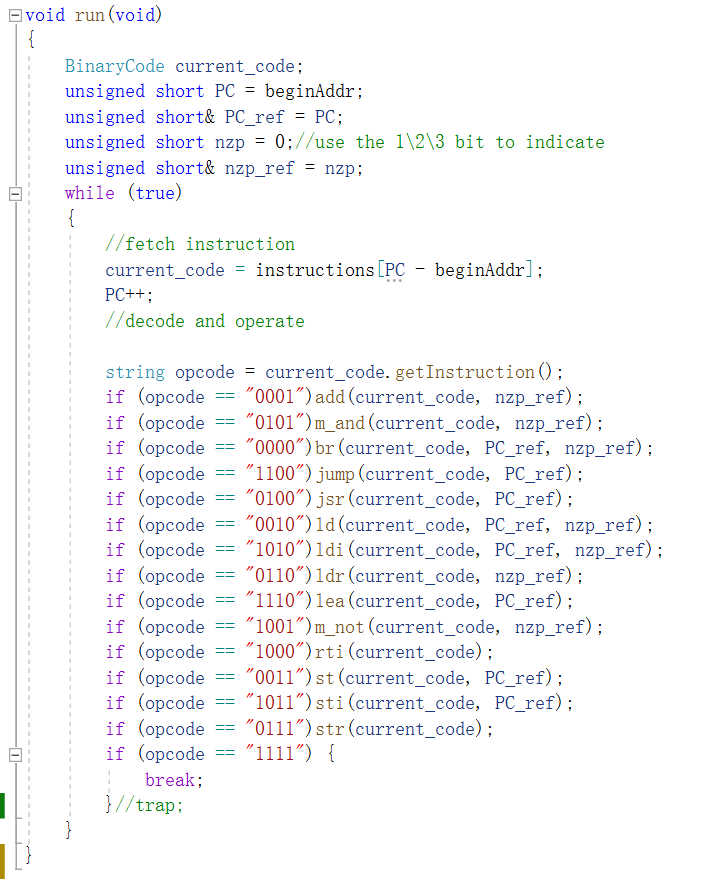
\includegraphics[width=0.7\textwidth]{decode and run.png}
		\caption{Fig 1} %名字
	\end{figure}
	
	
	
	\begin{figure}[htbp]
		\small
		\centering
		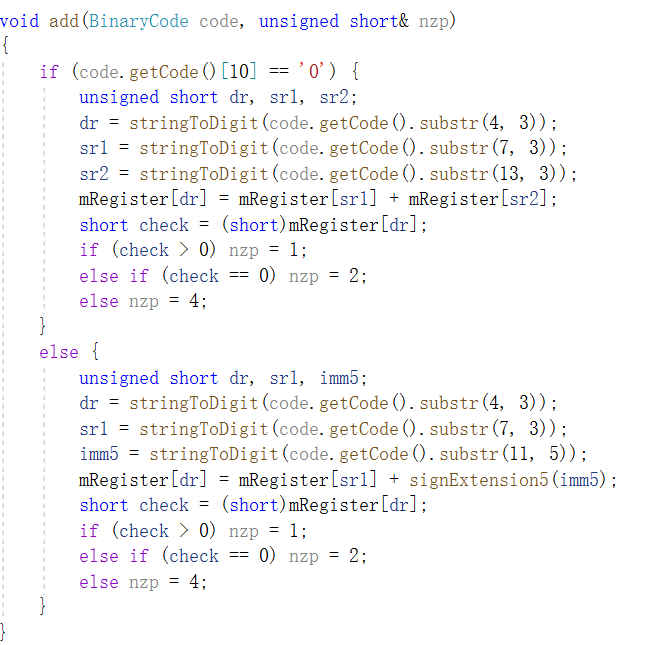
\includegraphics[width=0.7\textwidth]{add.png}
		\caption{Fig 2} %名字
	\end{figure}


	\begin{figure}[htbp]
		\small
		\centering
		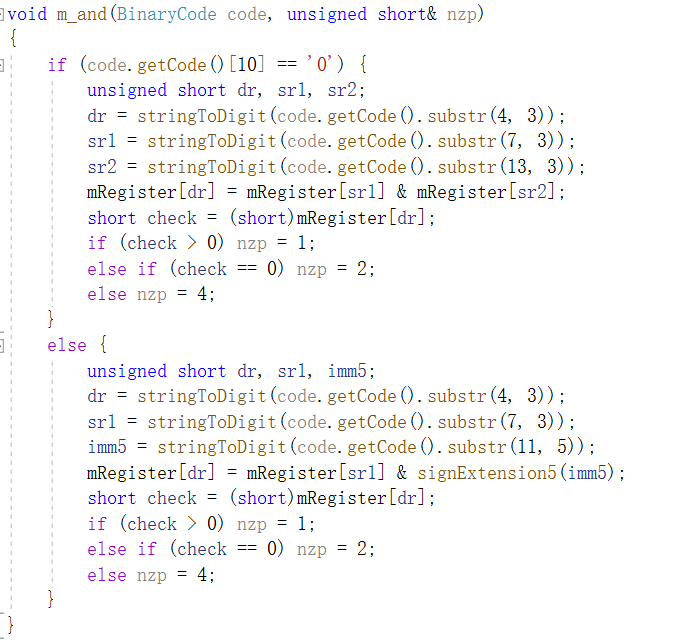
\includegraphics[width=0.7\textwidth]{and.png}
		\caption{Fig 3} %名字
	\end{figure}


	\begin{figure}[htbp]
		\small
		\centering
		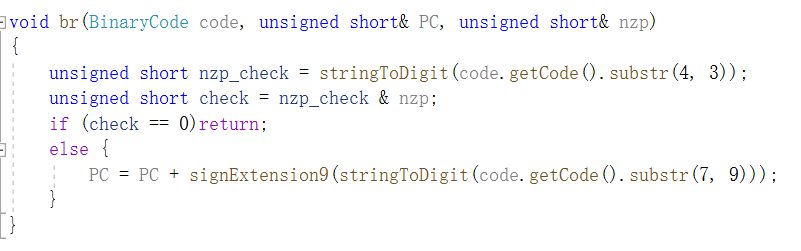
\includegraphics[width=0.7\textwidth]{br.png}
		\caption{Fig 4} %名字
	\end{figure}

	
	\begin{figure}[htbp]
		\small
		\centering
		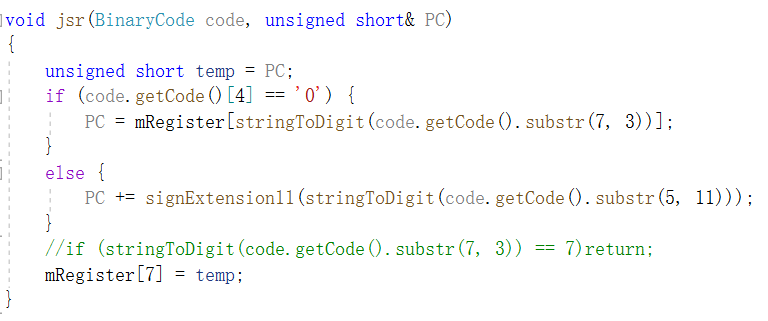
\includegraphics[width=0.7\textwidth]{jsr.png}
		\caption{Fig 5} %名字
	\end{figure}

	
	\begin{figure}[htbp]
		\small
		\centering
		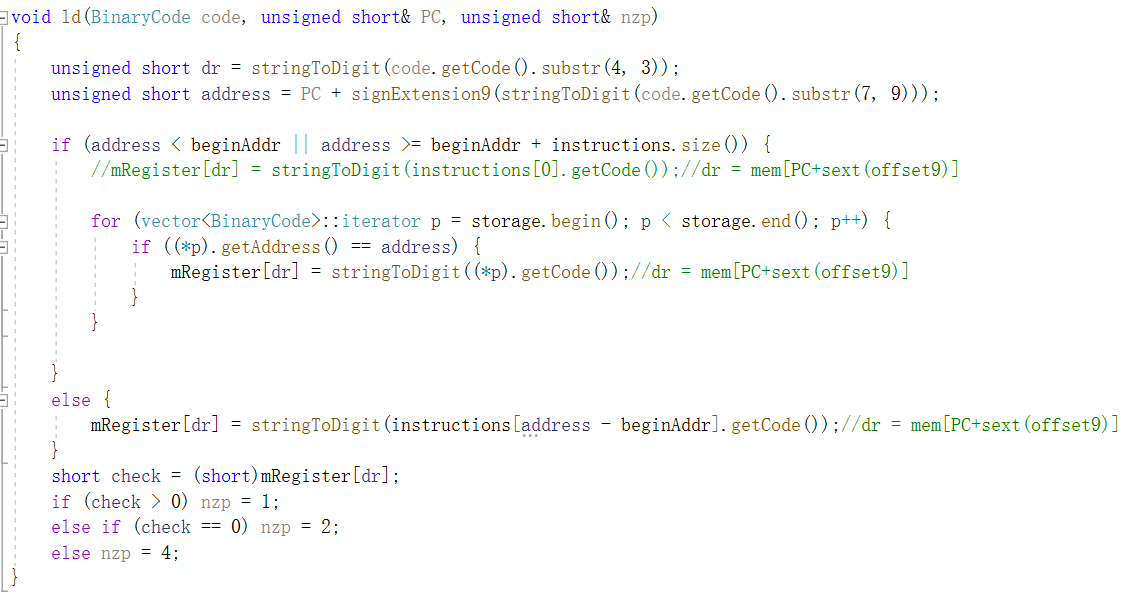
\includegraphics[width=0.7\textwidth]{load.png}
		\caption{Fig 6} %名字
	\end{figure}

	
	\begin{figure}[htbp]
		\small
		\centering
		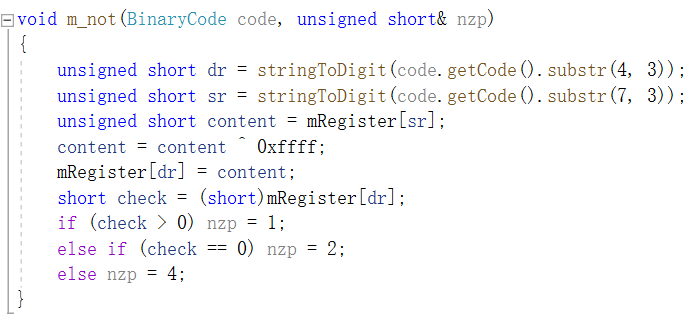
\includegraphics[width=0.7\textwidth]{not.png}
		\caption{Fig 7} %名字
	\end{figure}


	\begin{figure}[htbp]
		\small
		\centering
		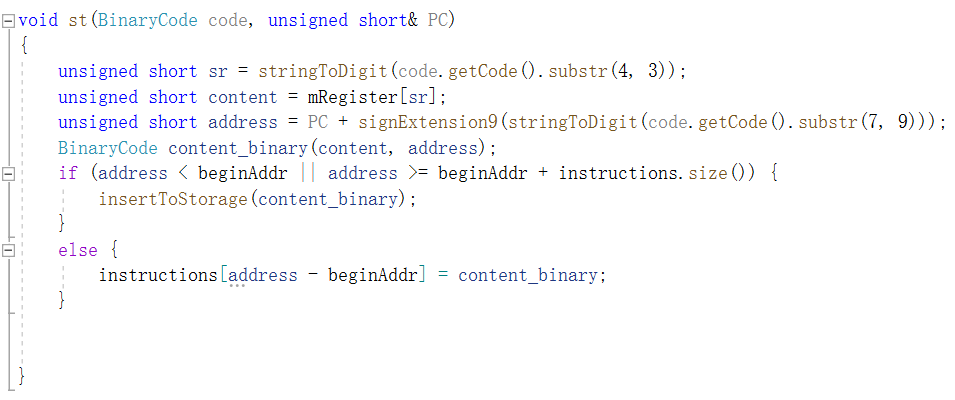
\includegraphics[width=0.7\textwidth]{store.png}
		\caption{Fig 8} %名字
	\end{figure}
	


\end{CJK*}
\end{document}





